\documentclass[]{article}
\usepackage{lmodern}
\usepackage{amssymb,amsmath}
\usepackage{ifxetex,ifluatex}
\usepackage{fixltx2e} % provides \textsubscript
\ifnum 0\ifxetex 1\fi\ifluatex 1\fi=0 % if pdftex
  \usepackage[T1]{fontenc}
  \usepackage[utf8]{inputenc}
\else % if luatex or xelatex
  \ifxetex
    \usepackage{mathspec}
  \else
    \usepackage{fontspec}
  \fi
  \defaultfontfeatures{Ligatures=TeX,Scale=MatchLowercase}
\fi
% use upquote if available, for straight quotes in verbatim environments
\IfFileExists{upquote.sty}{\usepackage{upquote}}{}
% use microtype if available
\IfFileExists{microtype.sty}{%
\usepackage{microtype}
\UseMicrotypeSet[protrusion]{basicmath} % disable protrusion for tt fonts
}{}
\usepackage[margin=1in]{geometry}
\usepackage{hyperref}
\hypersetup{unicode=true,
            pdftitle={OSF Supplementary Information},
            pdfauthor={Travis Riddle \& Stacey Sinclair},
            pdfborder={0 0 0},
            breaklinks=true}
\urlstyle{same}  % don't use monospace font for urls
\usepackage{longtable,booktabs}
\usepackage{graphicx,grffile}
\makeatletter
\def\maxwidth{\ifdim\Gin@nat@width>\linewidth\linewidth\else\Gin@nat@width\fi}
\def\maxheight{\ifdim\Gin@nat@height>\textheight\textheight\else\Gin@nat@height\fi}
\makeatother
% Scale images if necessary, so that they will not overflow the page
% margins by default, and it is still possible to overwrite the defaults
% using explicit options in \includegraphics[width, height, ...]{}
\setkeys{Gin}{width=\maxwidth,height=\maxheight,keepaspectratio}
\IfFileExists{parskip.sty}{%
\usepackage{parskip}
}{% else
\setlength{\parindent}{0pt}
\setlength{\parskip}{6pt plus 2pt minus 1pt}
}
\setlength{\emergencystretch}{3em}  % prevent overfull lines
\providecommand{\tightlist}{%
  \setlength{\itemsep}{0pt}\setlength{\parskip}{0pt}}
\setcounter{secnumdepth}{5}
% Redefines (sub)paragraphs to behave more like sections
\ifx\paragraph\undefined\else
\let\oldparagraph\paragraph
\renewcommand{\paragraph}[1]{\oldparagraph{#1}\mbox{}}
\fi
\ifx\subparagraph\undefined\else
\let\oldsubparagraph\subparagraph
\renewcommand{\subparagraph}[1]{\oldsubparagraph{#1}\mbox{}}
\fi

%%% Use protect on footnotes to avoid problems with footnotes in titles
\let\rmarkdownfootnote\footnote%
\def\footnote{\protect\rmarkdownfootnote}

%%% Change title format to be more compact
\usepackage{titling}

% Create subtitle command for use in maketitle
\newcommand{\subtitle}[1]{
  \posttitle{
    \begin{center}\large#1\end{center}
    }
}

\setlength{\droptitle}{-2em}
  \title{OSF Supplementary Information}
  \pretitle{\vspace{\droptitle}\centering\huge}
  \posttitle{\par}
  \author{Travis Riddle \& Stacey Sinclair}
  \preauthor{\centering\large\emph}
  \postauthor{\par}
  \predate{\centering\large\emph}
  \postdate{\par}
  \date{5/7/2018}

\usepackage{booktabs}
\usepackage{longtable}
\usepackage{array}
\usepackage{multirow}
\usepackage[table]{xcolor}
\usepackage{wrapfig}
\usepackage{float}
\usepackage{colortbl}
\usepackage{pdflscape}
\usepackage{tabu}
\usepackage{threeparttable}
\usepackage{threeparttablex}
\usepackage[normalem]{ulem}
\usepackage{makecell}

\usepackage{amsthm}
\newtheorem{theorem}{Theorem}[section]
\newtheorem{lemma}{Lemma}[section]
\theoremstyle{definition}
\newtheorem{definition}{Definition}[section]
\newtheorem{corollary}{Corollary}[section]
\newtheorem{proposition}{Proposition}[section]
\theoremstyle{definition}
\newtheorem{example}{Example}[section]
\theoremstyle{remark}
\newtheorem*{remark}{Remark}
\begin{document}
\maketitle

\section{Session details}\label{session-details}

Data analysis was done in R (R Core Team 2016) version 3.3.2 running
under OS X 10.11.6. Post-stratification was done with lme4, version
1.1.14 (Bates et al. 2015). Final model fitting was done on the
university cluster running Springdale Linux, release 6.9 using rstanarm,
version 2.17.2 (Stan Development Team 2016). We used the implementation
of the consensus monte carlo algorithm found in parallelMCMCcombine,
version 1.0 (Miroshnikov and Conlon 2014). Figures were made with
ggplot2, version 2.2.1 (Wickham 2009), with data manipulation done using
dplyr version 0.7.2 (Wickham et al. 2017) and tidyr, version 0.7.1
(Wickham and Henry 2017). Session info for computations on the local
machine is as follows:

\begin{verbatim}
## R version 3.3.2 (2016-10-31)
## Platform: x86_64-apple-darwin13.4.0 (64-bit)
## Running under: OS X El Capitan 10.11.6
## 
## locale:
## [1] en_US.UTF-8/en_US.UTF-8/en_US.UTF-8/C/en_US.UTF-8/en_US.UTF-8
## 
## attached base packages:
## [1] stats     graphics  grDevices utils     datasets  methods   base     
## 
## other attached packages:
## [1] bindrcpp_0.2     stringr_1.2.0    kableExtra_0.8.0 tidyr_0.7.1     
## [5] forcats_0.3.0    haven_1.0.0      ggplot2_2.2.1    dplyr_0.7.4     
## [9] knitr_1.20      
## 
## loaded via a namespace (and not attached):
##  [1] Rcpp_0.12.14      plyr_1.8.4        bindr_0.1        
##  [4] tools_3.3.2       digest_0.6.13     viridisLite_0.3.0
##  [7] evaluate_0.10     tibble_1.3.4      gtable_0.2.0     
## [10] pkgconfig_2.0.1   rlang_0.2.0.9000  rstudioapi_0.6   
## [13] yaml_2.1.14       httr_1.3.1        xml2_1.1.1       
## [16] rprojroot_1.2     grid_3.3.2        glue_1.1.1       
## [19] R6_2.2.2          rmarkdown_1.9     bookdown_0.4     
## [22] purrr_0.2.4       readr_1.0.0       magrittr_1.5     
## [25] codetools_0.2-15  backports_1.0.5   scales_0.5.0.9000
## [28] htmltools_0.3.6   assertthat_0.2.0  rvest_0.3.2      
## [31] colorspace_1.3-2  stringi_1.1.2     lazyeval_0.2.1   
## [34] munsell_0.4.3
\end{verbatim}

Session info for the computations run on the university cluster is as
follows:

\begin{verbatim}
R version 3.4.3 (2017-11-30)
Platform: x86_64-redhat-linux-gnu (64-bit)
Running under: Springdale Linux 7.4 (Verona)

Matrix products: default
BLAS/LAPACK: /usr/lib64/R/lib/libRblas.so

locale:
 [1] LC_CTYPE=en_US.UTF-8       LC_NUMERIC=C
 [3] LC_TIME=en_US.UTF-8        LC_COLLATE=en_US.UTF-8
 [5] LC_MONETARY=en_US.UTF-8    LC_MESSAGES=en_US.UTF-8
 [7] LC_PAPER=en_US.UTF-8       LC_NAME=C
 [9] LC_ADDRESS=C               LC_TELEPHONE=C
[11] LC_MEASUREMENT=en_US.UTF-8 LC_IDENTIFICATION=C

attached base packages:
[1] stats     graphics  grDevices utils     datasets  methods   base

other attached packages:
[1] rstanarm_2.15.3 Rcpp_0.12.13    ggplot2_2.2.1   forcats_0.2.0
[5] tidyr_0.7.2     dplyr_0.7.4

loaded via a namespace (and not attached):
 [1] lattice_0.20-35      zoo_1.8-0            gtools_3.5.0
 [4] assertthat_0.2.0     digest_0.6.12        mime_0.5
 [7] R6_2.2.2             plyr_1.8.4           stats4_3.4.3
[10] colourpicker_1.0     rlang_0.1.2          lazyeval_0.2.1
[13] minqa_1.2.4          miniUI_0.1.1         nloptr_1.0.4
[16] Matrix_1.2-12        DT_0.2               shinythemes_1.1.1
[19] splines_3.4.3        shinyjs_0.9.1        lme4_1.1-14
[22] stringr_1.2.0        htmlwidgets_0.9      loo_1.1.0
[25] igraph_1.1.2         munsell_0.4.3        shiny_1.0.5
[28] compiler_3.4.3       httpuv_1.3.5         rstan_2.16.2
[31] pkgconfig_2.0.1      base64enc_0.1-3      rstantools_1.3.0
[34] htmltools_0.3.6      tibble_1.3.4         gridExtra_2.3
[37] threejs_0.3.1        codetools_0.2-15     matrixStats_0.52.2
[40] MASS_7.3-47          grid_3.4.3           nlme_3.1-131
[43] xtable_1.8-2         gtable_0.2.0         magrittr_1.5
[46] StanHeaders_2.16.0-1 scales_0.5.0         stringi_1.1.5
[49] reshape2_1.4.2       bindrcpp_0.2         dygraphs_1.1.1.4
[52] xts_0.10-0           tools_3.4.3          glue_1.2.0
[55] shinystan_2.4.0      markdown_0.8         purrr_0.2.4
[58] crosstalk_1.0.0      rsconnect_0.8.5      parallel_3.4.3
[61] inline_0.3.14        colorspace_1.3-2     bayesplot_1.4.0
[64] bindr_0.1
\end{verbatim}

\section{Preregistered analysis}\label{preregistered-analysis}

Here, we describe, in detail, the differences between the registered
analysis plan and that presented in the main text, along with our
reasons for making the alterations.

\subsection{Data exclusions}\label{data-exclusions}

In our preanalysis plan, we specified our analyses to focus on 13
actions - corporal punishment, in-school suspension, out-of-school
suspension, expulsion with educational services, expulsion without
educational services, expulsion under zero-tolerance policies, referral
to law enforcement, school-related arrests, mechanical restraint,
physical restraint, seclusion, preschool suspension, and preschool
expulsion. However, upon further study, we discovered reasons we thought
justified excluding a number of these outcomes.

First, seclusion, physical restraint, and mechanical restraint are not
disciplinary actions, but are rather used as means to restrain students
who are at risk of harming themselves or others.

Next, we discovered that the administration of corporal punishment was
extremely irregular across counties, with almost all cases ocurring in
the South. Specifically, Alabama, Arkansas, Florida, Georgia, Louisiana,
Missouri, Mississippi, Oklahoma, Tennessee, and Texas accounted for 98\%
of all educational institutions that administered corporal punishment at
least once, despite containing only 26.9\% of the educational
institutions in the full dataset. It is not clear whether this uneven
distribution is due to legal prohibitions, cultural differences, or some
combination of the two. Because this makes interpretation of the
parameters uncertain, this analysis is also placed in the appendix.

We also found that the number of preschool students who are expelled or
suspended is vanishingly small (131 total expulsions and 6751 total
suspensions out of over 1.4 million enrolled preschool students), making
reliably estimating any association across counties exceedingly
unlikely. We additionally discovered that counts of one expulsion
category (expulsion under zero-tolerance policies) overlapped with
counts in other categories, and so excluded this category from the main
text. We also decided to combine the remaining two expulsion categories
to yield one overall count of the number of students expelled. We did
this to remain consistent with previous research, and to obtain
district-level rates of expulsion that were slightly higher, and
therefore more amenable to exploring variation across counties.

When preparing the preregistration, we also had not known about the
issues with juvenile justice facilities, or with the school districts
with reporting errors, and so excluded these schools from analyses in
the main text.

\subsection{Changes in measurement \& estimation of
bias}\label{changes-in-measurement-estimation-of-bias}

We preregistered our explicit bias as a simple feeling thermometer
towards balcks (i.e. \emph{how warm or cold do you feel towards Blacks?
0=very cold, 10=very warm}). However, the majority of past research (see
for example Leitner et al. (2016) and Hehman, Flake, and Calanchini
(2017)) has used the difference in reported warmth towards whites and
blacks, and so in the main text, we report models using this metric of
explicit bias.

Our main text presents analyses with poststratified estimates of bias.
Our registered analysis also described analyses with raw, county-based
means. Unlike previous papers that used poststratification, we see
substantial differences in results between the two estimation methods.
Because post-stratification is known to yield better estimates, we
suspect that the difference in results is largely driven by extreme
county-level observations with little data to support these extreme
estimates. Nevertheless, in the interest of completion, we present the
model using raw county-level means as well.

We also registered an exploratory analysis using the responses of people
who visited Project Implicit and identified themselves as teachers.
Unfortunately, without population-level data on the demographic
characteristics of teachers, we are not able to post-stratify these
estimates. Additionally, there were relatively few teachers in the
Project Implicit from which to derive estimates. Ultimately, we have
little confidence that this analysis tells us anything about whether the
biases of teachers specifically contribute to disparities in
disciplinary actions, and so this analysis is also limited to the
appendix.

\subsection{Additional covariates}\label{additional-covariates}

We included four covariates that were not specified in the registered
analysis. Specifically, the mobility, housing density, crime rate, and
dissimilarity covariates. We also interacted all covariates with race.
These modifications were done in order to cover more of the covariates
that were included in previous papers (Leitner et al. 2016).

\section{Registered analysis results}\label{registered-analysis-results}

Here, we present the results of the preregistered analyses exactly.
Though we described a number of changes above, it is not practical to
run all possible combination of changes, as each set of models takes
several days to just to estimate, and there are at least several dozen
possible combinations of decisions to test, depending on how
fine-grained one wishes to be with the decisions. Accordingly, we limit
the presentation of results below to just the three models that we
registered.

\subsection{County-level estimates}\label{county-level-estimates}

\begin{figure}
\centering
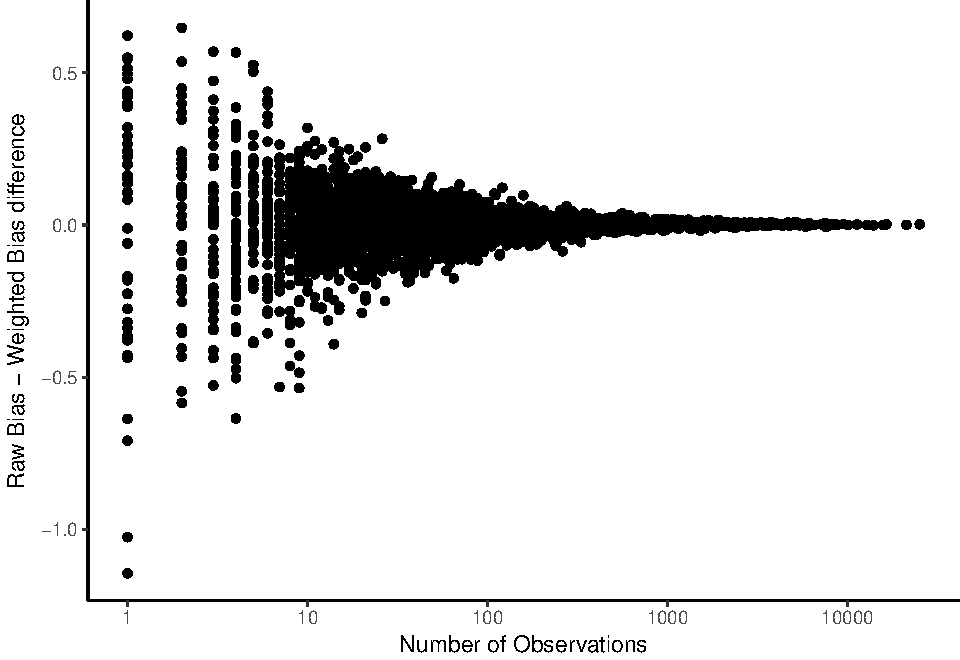
\includegraphics{osf_supplement_files/figure-latex/raw-county-estimates-1.pdf}
\caption{\label{fig:raw-county-estimates}\label{fig:raw-county-estimates}Difference
in raw county means and post-stratifed estimates of implicit bias as a
function of the number of observations in each county. The X axis is on
the log scale.}
\end{figure}

Examining the models fit with simple county means, we find that the
county-level estimates vary more than with the post-stratified
estimates. This pattern is expected, as one desireable feature of
post-stratification is that it regularizes extreme observations without
a large amount of data to support them. This phenomena is illustrated in
figure \ref{fig:raw-county-estimates}, which shows the distribution of
differences between the raw county means and the post-stratified
estimates of implicit bias as a function of the number of observations
in each county. More specifically, while the mean of the county-level
means does not meaningfully differ from the post-stratified estimates,
the standard deviation is much larger (\(M_{implicit}\) = 0.4,
\(SD_{implicit}\) = 0.11; \(M_{explicit}\) = 6.24, \(SD_{explicit}\) =
0.59)\footnote{This explicit estimate is based on the simple warmth
  towards blacks question, and not the difference between warmth towards
  whites and warmth twoards blacks.}

The county-level implicit bias estimates for the poststratified model
are as reported in the main text. The estimates for explicit bias are
slightly different, as they are not computed based on the difference in
reporting warmth toward whites and warmth toward blacks. Specifically,
the average amount of bias at the county-level is 6.25 (SD = 0.14).

A subset of years in the Project Implicit data also collected
occupational information from respondents. As identified in our
pre-analysis plan, we took advantage of the presence of primary and
secondary educators in these data to test whether any associations
between bias and race-based differences in the rates of disciplinary
action were stronger among these respondents. Filtering for only white
individuals who identified as primary, secondary, special education, and
other teachers and instructors (occupation codes 25-2000 and 25-3000)
reduced the dataset to 76959 respondents. In order to assure that our
estimates were reasonably stable, we limited analysis to only counties
that had at least 50 respondents. As such, our teacher analysis is
limited to just 327 counties. Additionally, because we do not know of
any state-level demographic estimates for teachers, we were unable to
perform post-stratification for these data. Nonetheless, across these
limited counties, the overall estimate of implicit and explicit bias are
similar to those for the whole dataset (\(M_{implicit}\) = 0.37,
\(SD_{implicit}\) = 0.06; \(M_{explicit}\) = 6.68, \(SD_{explicit}\) =
0.27).

For all models, explicit and implicit bias were scored such that higher
scores reflect a greater preference for whites/reduced preference for
blacks.

\subsection{Model estimates}\label{model-estimates}

Tables \ref{tab:mod-raw-table1} and \ref{tab:mod-raw-table2} present
results from the model fit to the raw, county-level means (we broke
results from each set of estimates into two table to improve
legibility). The table presents parameter estimates (operationalized as
the mean of the posterior) and 95\% uncertainty intervals for each of
the population-level effects for each of the outcomes. Tables
\ref{tab:mod-post-table1} and \ref{tab:mod-post-table2} present the
results for post-stratified estimates, with tables
\ref{tab:mod-teach-table1} and \ref{tab:mod-teach-table2} showing
results for the teacher models.

\begin{landscape}\begin{table}

\caption{\label{tab:mod-raw-table1}\label{tab:model-raw-table1}Regression coefficient estimates for the population-level (i.e. fixed) effects, 
             along with 95\% uncertainty intervals for each of the disciplinary metrics. Model uses raw 
             county-means as bias estimates.}
\centering
\resizebox{\linewidth}{!}{\begin{tabular}[t]{lllllll}
\toprule
 & Seclusion & \makecell[l]{Physical\\Restraint} & \makecell[l]{Mechanical\\Restraint} & \makecell[l]{Corporal\\Punishment} & \makecell[l]{Preschool\\Suspension} & \makecell[l]{Preschool\\Expulsion}\\
\midrule
Intercept & \textbf{-11.19 [-11.64,-10.76]} & \textbf{-8.78 [-9,-8.58]} & \textbf{-14.1 [-14.98,-13.31]} & \textbf{-3.21 [-3.31,-3.13]} & \textbf{-8.84 [-9.16,-8.56]} & \textbf{-16.07 [-17.98,-14.37]}\\
proportion black & \textbf{-1.51 [-2.19,-0.83]} & \textbf{-0.67 [-1.04,-0.31]} & 0.8 [-0.13,1.75] & 0.11 [-0.15,0.37] & \textbf{1.02 [0.6,1.46]} & 0.99 [-0.51,2.52]\\
proportion white & 0.26 [-0.2,0.73] & 0.19 [-0.08,0.45] & 0.26 [-0.5,1.04] & \textbf{-0.3 [-0.5,-0.08]} & \textbf{-0.44 [-0.8,-0.07]} & -0.34 [-1.54,0.95]\\
black-white ratio & \textbf{0.81 [0.15,1.44]} & 0.26 [-0.08,0.6] & -0.59 [-1.47,0.26] & \textbf{-0.34 [-0.52,-0.15]} & \textbf{-0.78 [-1.14,-0.44]} & -0.34 [-1.61,0.81]\\
total population & \textbf{0.16 [0,0.31]} & 0.02 [-0.07,0.12] & \textbf{0.41 [0.21,0.64]} & \textbf{-0.48 [-0.67,-0.3]} & 0.05 [-0.06,0.17] & \textbf{0.49 [0.24,0.77]}\\
\addlinespace
college grads & \textbf{0.25 [0.01,0.49]} & \textbf{0.3 [0.17,0.43]} & -0.04 [-0.47,0.36] & \textbf{-0.15 [-0.24,-0.05]} & \textbf{-0.21 [-0.4,-0.02]} & -0.24 [-0.96,0.45]\\
income & \textbf{-0.32 [-0.63,-0.02]} & -0.18 [-0.37,0] & 0 [-0.53,0.53] & \textbf{-0.33 [-0.48,-0.18]} & \textbf{-0.3 [-0.57,-0.03]} & -0.35 [-1.33,0.56]\\
poverty & \textbf{-0.64 [-1.05,-0.22]} & -0.14 [-0.37,0.09] & 0.3 [-0.34,0.95] & 0.01 [-0.15,0.17] & \textbf{-0.32 [-0.65,0]} & \textbf{-1.21 [-2.46,-0.03]}\\
unemployment & \textbf{0.4 [0.15,0.68]} & \textbf{0.23 [0.08,0.38]} & -0.21 [-0.65,0.23] & \textbf{-0.14 [-0.23,-0.05]} & \textbf{-0.29 [-0.48,-0.09]} & -0.3 [-1.12,0.53]\\
implicit bias & -0.02 [-0.38,0.36] & 0 [-0.23,0.22] & -0.07 [-0.59,0.46] & -0.01 [-0.1,0.08] & -0.16 [-0.4,0.07] & 0.04 [-0.96,1.09]\\
\addlinespace
explicit bias & 0.33 [-0.04,0.69] & 0.07 [-0.13,0.28] & -0.14 [-0.65,0.37] & -0.06 [-0.15,0.03] & -0.17 [-0.41,0.06] & -0.05 [-1.11,0.99]\\
race: white & \textbf{-1.04 [-1.39,-0.67]} & \textbf{-1.01 [-1.19,-0.82]} & \textbf{-1.72 [-2.36,-1.05]} & \textbf{-0.68 [-0.73,-0.62]} & \textbf{-1.65 [-1.95,-1.35]} & \textbf{-1.91 [-3.45,-0.41]}\\
implicit bias*race: white & 0.12 [-0.24,0.49] & 0.08 [-0.15,0.3] & 0.06 [-0.45,0.57] & -0.04 [-0.1,0.03] & 0.2 [-0.06,0.46] & -0.03 [-1.28,1.19]\\
explicit bias*race: white & -0.22 [-0.57,0.14] & -0.01 [-0.21,0.2] & -0.09 [-0.61,0.42] & 0 [-0.06,0.06] & 0.08 [-0.17,0.35] & -0.4 [-1.72,0.88]\\
\bottomrule
\end{tabular}}
\end{table}
\end{landscape}

\begin{landscape}\begin{table}

\caption{\label{tab:mod-raw-table2}\label{tab:model-raw-table1}Regression coefficient estimates for the population-level (i.e. fixed) effects, 
             along with 95\% uncertainty intervals for each of the disciplinary metrics. Model uses raw 
             county-means as bias estimates.}
\centering
\resizebox{\linewidth}{!}{\begin{tabular}[t]{llllllll}
\toprule
 & \makecell[l]{Out-of-School\\Suspension} & \makecell[l]{Law Enf.\\Referral} & \makecell[l]{In-School\\Suspension} & \makecell[l]{School-Related\\Arrest} & \makecell[l]{Expulsion w/o\\ Ed. Services} & \makecell[l]{Expulsion w/Ed.\\Services} & \makecell[l]{Expulsion Under\\Zero-Tolerance}\\
\midrule
Intercept & \textbf{-2.68 [-2.71,-2.65]} & \textbf{-6.12 [-6.2,-6.03]} & \textbf{-2.63 [-2.67,-2.59]} & \textbf{-8.2 [-8.37,-8.04]} & \textbf{-8.22 [-8.39,-8.06]} & \textbf{-8.11 [-8.28,-7.95]} & \textbf{-9.74 [-10,-9.49]}\\
proportion black & \textbf{0.34 [0.27,0.42]} & \textbf{-0.45 [-0.64,-0.26]} & \textbf{0.61 [0.51,0.71]} & -0.19 [-0.5,0.13] & \textbf{0.32 [0.03,0.62]} & -0.29 [-0.6,0.02] & 0.02 [-0.36,0.42]\\
proportion white & 0.02 [-0.03,0.08] & \textbf{-0.34 [-0.48,-0.2]} & \textbf{0.13 [0.05,0.21]} & -0.06 [-0.3,0.19] & 0.23 [-0.03,0.48] & \textbf{-0.25 [-0.47,-0.02]} & 0.21 [-0.09,0.52]\\
black-white ratio & \textbf{-0.21 [-0.27,-0.15]} & 0.06 [-0.1,0.23] & \textbf{-0.53 [-0.62,-0.45]} & 0.09 [-0.17,0.35] & -0.13 [-0.35,0.09] & -0.22 [-0.53,0.08] & -0.23 [-0.61,0.14]\\
total population & 0.01 [-0.02,0.03] & 0.01 [-0.06,0.07] & -0.03 [-0.07,0] & 0.09 [0,0.19] & 0.01 [-0.08,0.1] & 0.06 [-0.03,0.16] & 0.09 [-0.02,0.2]\\
\addlinespace
college grads & \textbf{-0.04 [-0.07,-0.01]} & 0.03 [-0.06,0.11] & \textbf{-0.12 [-0.16,-0.07]} & \textbf{0.15 [0.01,0.29]} & \textbf{-0.2 [-0.34,-0.06]} & -0.06 [-0.19,0.07] & -0.08 [-0.26,0.09]\\
income & \textbf{-0.09 [-0.14,-0.05]} & -0.05 [-0.16,0.06] & \textbf{-0.08 [-0.14,-0.02]} & 0 [-0.18,0.17] & \textbf{-0.31 [-0.49,-0.13]} & -0.09 [-0.26,0.09] & -0.08 [-0.3,0.14]\\
poverty & 0.02 [-0.03,0.08] & \textbf{-0.4 [-0.53,-0.27]} & \textbf{0.2 [0.12,0.26]} & \textbf{-0.22 [-0.44,0]} & \textbf{-0.35 [-0.57,-0.13]} & -0.15 [-0.38,0.06] & 0.2 [-0.07,0.46]\\
unemployment & \textbf{0.22 [0.18,0.25]} & \textbf{0.19 [0.1,0.27]} & 0.03 [-0.01,0.07] & \textbf{0.25 [0.1,0.4]} & \textbf{0.45 [0.31,0.59]} & \textbf{0.27 [0.13,0.41]} & \textbf{0.31 [0.14,0.48]}\\
implicit bias & 0.01 [-0.03,0.05] & -0.06 [-0.17,0.04] & \textbf{0.08 [0.03,0.12]} & -0.09 [-0.26,0.1] & 0.04 [-0.12,0.21] & -0.1 [-0.28,0.08] & -0.03 [-0.27,0.21]\\
\addlinespace
explicit bias & 0.03 [-0.01,0.06] & 0.09 [-0.01,0.19] & 0 [-0.04,0.04] & -0.02 [-0.19,0.15] & -0.01 [-0.17,0.14] & 0.02 [-0.14,0.19] & \textbf{0.3 [0.08,0.52]}\\
race: white & \textbf{-1.06 [-1.09,-1.03]} & \textbf{-0.83 [-0.9,-0.77]} & \textbf{-0.85 [-0.87,-0.82]} & \textbf{-1.07 [-1.18,-0.94]} & \textbf{-0.88 [-1.02,-0.74]} & \textbf{-0.85 [-0.98,-0.72]} & \textbf{-0.49 [-0.71,-0.27]}\\
implicit bias*race: white & -0.01 [-0.04,0.03] & -0.03 [-0.13,0.06] & \textbf{-0.04 [-0.07,-0.01]} & 0.01 [-0.16,0.16] & -0.09 [-0.24,0.05] & 0.11 [-0.04,0.26] & -0.19 [-0.41,0.04]\\
explicit bias*race: white & 0 [-0.03,0.03] & \textbf{-0.1 [-0.18,-0.01]} & -0.02 [-0.05,0.01] & -0.02 [-0.17,0.12] & 0 [-0.14,0.14] & -0.02 [-0.17,0.12] & -0.14 [-0.34,0.07]\\
\bottomrule
\end{tabular}}
\end{table}
\end{landscape}

\begin{landscape}\begin{table}

\caption{\label{tab:mod-post-table1}\label{tab:model-post-table1}Regression coefficient estimates for the 
             population-level (i.e. fixed) effects, along with 95\% 
             uncertainty intervals for each of the disciplinary metrics. 
             Model uses bias estimates as derived from poststratification 
             scheme.}
\centering
\resizebox{\linewidth}{!}{\begin{tabular}[t]{lllllll}
\toprule
 & Seclusion & \makecell[l]{Physical\\Restraint} & \makecell[l]{Mechanical\\Restraint} & \makecell[l]{Corporal\\Punishment} & \makecell[l]{Preschool\\Suspension} & \makecell[l]{Preschool\\Expulsion}\\
\midrule
Intercept & \textbf{-11.11 [-11.55,-10.7]} & \textbf{-8.73 [-8.94,-8.53]} & \textbf{-13.96 [-14.8,-13.17]} & \textbf{-3.24 [-3.33,-3.15]} & \textbf{-9 [-9.35,-8.69]} & \textbf{-14.17 [-15.97,-12.57]}\\
proportion black & \textbf{-0.79 [-1.45,-0.11]} & -0.4 [-0.8,0.02] & 0.86 [-0.19,1.9] & 0.13 [-0.17,0.41] & \textbf{0.78 [0.32,1.25]} & 0.58 [-0.89,2.15]\\
proportion white & \textbf{0.49 [0.02,0.99]} & \textbf{0.28 [0,0.56]} & 0.18 [-0.6,0.99] & \textbf{-0.25 [-0.47,-0.02]} & \textbf{-0.56 [-0.91,-0.19]} & -0.7 [-1.84,0.56]\\
black-white ratio & 0.52 [-0.08,1.06] & 0.15 [-0.26,0.52] & -0.84 [-1.95,0.14] & \textbf{-0.33 [-0.51,-0.14]} & \textbf{-0.76 [-1.13,-0.4]} & -0.37 [-1.88,0.84]\\
total population & \textbf{0.14 [0.01,0.28]} & 0.03 [-0.06,0.11] & \textbf{0.32 [0.14,0.52]} & \textbf{-0.44 [-0.62,-0.26]} & 0.03 [-0.06,0.13] & 0.22 [0,0.45]\\
\addlinespace
college grads & 0.2 [-0.04,0.45] & \textbf{0.27 [0.14,0.41]} & -0.02 [-0.43,0.39] & \textbf{-0.12 [-0.22,-0.02]} & -0.12 [-0.32,0.07] & -0.2 [-0.92,0.48]\\
income & -0.27 [-0.56,0.04] & -0.17 [-0.34,0.01] & 0.03 [-0.48,0.55] & \textbf{-0.38 [-0.53,-0.22]} & \textbf{-0.38 [-0.64,-0.12]} & -0.15 [-1.03,0.71]\\
poverty & \textbf{-0.55 [-0.96,-0.14]} & -0.14 [-0.38,0.1] & 0.3 [-0.37,0.94] & 0 [-0.17,0.16] & \textbf{-0.44 [-0.76,-0.12]} & -1.02 [-2.21,0.12]\\
unemployment & \textbf{0.44 [0.18,0.71]} & \textbf{0.26 [0.11,0.42]} & -0.17 [-0.6,0.27] & \textbf{-0.12 [-0.21,-0.02]} & \textbf{-0.21 [-0.41,-0.02]} & -0.21 [-1,0.56]\\
implicit bias & \textbf{-0.42 [-0.71,-0.14]} & \textbf{-0.33 [-0.51,-0.16]} & -0.07 [-0.51,0.41] & 0.01 [-0.11,0.13] & 0.14 [-0.09,0.39] & 0.01 [-1,1.02]\\
\addlinespace
explicit bias & 0.11 [-0.15,0.37] & -0.04 [-0.19,0.12] & -0.06 [-0.45,0.35] & \textbf{-0.14 [-0.24,-0.05]} & \textbf{-0.21 [-0.41,-0.02]} & -0.51 [-1.39,0.4]\\
race: white & \textbf{-1.06 [-1.4,-0.69]} & \textbf{-1.02 [-1.2,-0.82]} & \textbf{-1.77 [-2.44,-1.13]} & \textbf{-0.64 [-0.7,-0.57]} & \textbf{-1.6 [-1.92,-1.26]} & \textbf{-2.09 [-3.6,-0.61]}\\
implicit bias*race: white & -0.1 [-0.32,0.12] & \textbf{0.18 [0.05,0.31]} & -0.02 [-0.39,0.36] & \textbf{-0.11 [-0.18,-0.05]} & -0.06 [-0.28,0.16] & -0.72 [-1.93,0.46]\\
explicit bias*race: white & -0.15 [-0.37,0.07] & 0.03 [-0.11,0.16] & -0.32 [-0.65,0.03] & -0.02 [-0.08,0.05] & -0.13 [-0.32,0.07] & -0.48 [-1.64,0.63]\\
\bottomrule
\end{tabular}}
\end{table}
\end{landscape}

\begin{landscape}\begin{table}

\caption{\label{tab:mod-post-table2}\label{tab:model-post-table2}Regression coefficient estimates for the 
             population-level (i.e. fixed) effects, along with 95\% 
             uncertainty intervals for each of the disciplinary metrics. 
             Model uses bias estimates as derived from poststratification 
             scheme.}
\centering
\resizebox{\linewidth}{!}{\begin{tabular}[t]{llllllll}
\toprule
 & \makecell[l]{Out-of-School\\Suspension} & \makecell[l]{Law Enf.\\Referral} & \makecell[l]{In-School\\Suspension} & \makecell[l]{School-Related\\Arrest} & \makecell[l]{Expulsion w/o\\ Ed. Services} & \makecell[l]{Expulsion w/Ed.\\Services} & \makecell[l]{Expulsion Under\\Zero-Tolerance}\\
\midrule
Intercept & \textbf{-2.69 [-2.72,-2.66]} & \textbf{-6.12 [-6.21,-6.03]} & \textbf{-2.63 [-2.67,-2.59]} & \textbf{-8.19 [-8.36,-8.03]} & \textbf{-8.2 [-8.37,-8.03]} & \textbf{-8.09 [-8.26,-7.92]} & \textbf{-9.66 [-9.92,-9.4]}\\
proportion black & \textbf{0.28 [0.21,0.36]} & \textbf{-0.28 [-0.48,-0.08]} & \textbf{0.31 [0.2,0.41]} & -0.26 [-0.59,0.08] & \textbf{0.47 [0.14,0.79]} & \textbf{-0.37 [-0.72,-0.03]} & 0.17 [-0.25,0.59]\\
proportion white & 0 [-0.06,0.06] & \textbf{-0.29 [-0.43,-0.15]} & 0.07 [0,0.15] & -0.1 [-0.34,0.16] & \textbf{0.28 [0.01,0.56]} & \textbf{-0.26 [-0.5,-0.03]} & 0.27 [-0.03,0.58]\\
black-white ratio & \textbf{-0.19 [-0.24,-0.13]} & -0.01 [-0.17,0.15] & \textbf{-0.36 [-0.44,-0.28]} & 0.08 [-0.17,0.33] & -0.19 [-0.42,0.04] & -0.17 [-0.48,0.11] & -0.24 [-0.62,0.1]\\
total population & 0 [-0.03,0.02] & 0.02 [-0.04,0.08] & \textbf{-0.04 [-0.07,0]} & 0.09 [0,0.19] & 0 [-0.08,0.09] & 0.06 [-0.03,0.15] & 0.09 [-0.01,0.2]\\
\addlinespace
college grads & \textbf{-0.04 [-0.07,-0.01]} & -0.01 [-0.09,0.07] & \textbf{-0.08 [-0.12,-0.03]} & \textbf{0.17 [0.03,0.31]} & \textbf{-0.23 [-0.37,-0.09]} & -0.05 [-0.19,0.08] & -0.14 [-0.31,0.04]\\
income & \textbf{-0.09 [-0.14,-0.05]} & -0.03 [-0.14,0.08] & \textbf{-0.11 [-0.17,-0.05]} & -0.01 [-0.18,0.17] & \textbf{-0.29 [-0.47,-0.11]} & -0.11 [-0.28,0.07] & -0.06 [-0.28,0.17]\\
poverty & 0.02 [-0.03,0.07] & \textbf{-0.38 [-0.51,-0.25]} & \textbf{0.16 [0.09,0.23]} & -0.2 [-0.43,0.02] & \textbf{-0.3 [-0.52,-0.09]} & -0.17 [-0.39,0.04] & 0.23 [-0.04,0.5]\\
unemployment & \textbf{0.21 [0.18,0.25]} & \textbf{0.18 [0.09,0.26]} & \textbf{0.06 [0.01,0.1]} & \textbf{0.26 [0.11,0.41]} & \textbf{0.41 [0.28,0.55]} & \textbf{0.27 [0.13,0.42]} & \textbf{0.26 [0.09,0.44]}\\
implicit bias & \textbf{0.08 [0.04,0.13]} & -0.08 [-0.19,0.01] & \textbf{0.13 [0.08,0.19]} & 0 [-0.16,0.16] & -0.03 [-0.19,0.13] & -0.03 [-0.2,0.13] & -0.15 [-0.36,0.06]\\
\addlinespace
explicit bias & \textbf{0.06 [0.02,0.09]} & \textbf{0.12 [0.03,0.21]} & \textbf{-0.16 [-0.2,-0.11]} & -0.08 [-0.23,0.06] & \textbf{0.14 [0,0.28]} & -0.06 [-0.2,0.09] & \textbf{0.25 [0.06,0.43]}\\
race: white & \textbf{-1.05 [-1.08,-1.02]} & \textbf{-0.83 [-0.89,-0.76]} & \textbf{-0.84 [-0.86,-0.81]} & \textbf{-1.05 [-1.18,-0.92]} & \textbf{-0.9 [-1.04,-0.76]} & \textbf{-0.87 [-1,-0.73]} & \textbf{-0.53 [-0.75,-0.3]}\\
implicit bias*race: white & \textbf{-0.04 [-0.07,-0.01]} & -0.04 [-0.1,0.02] & \textbf{-0.04 [-0.07,-0.02]} & 0 [-0.09,0.09] & -0.02 [-0.12,0.09] & 0.09 [-0.01,0.18] & 0.07 [-0.08,0.22]\\
explicit bias*race: white & 0 [-0.03,0.03] & -0.04 [-0.1,0.01] & 0 [-0.03,0.02] & -0.02 [-0.1,0.07] & 0.02 [-0.08,0.12] & 0.04 [-0.05,0.12] & 0.02 [-0.11,0.16]\\
\bottomrule
\end{tabular}}
\end{table}
\end{landscape}

\begin{landscape}\begin{table}

\caption{\label{tab:mod-teach-table1}\label{tab:model-teach-table1}Regression coefficient estimates for the 
             population-level (i.e. fixed) effects, along with 95\% 
             uncertainty intervals for each of the disciplinary metrics. 
             Model uses only data from Project Implicit respondents who 
             identified as teachers.}
\centering
\resizebox{\linewidth}{!}{\begin{tabular}[t]{lllllll}
\toprule
 & Seclusion & \makecell[l]{Physical\\Restraint} & \makecell[l]{Mechanical\\Restraint} & \makecell[l]{Corporal\\Punishment} & \makecell[l]{Preschool\\Suspension} & \makecell[l]{Preschool\\Expulsion}\\
\midrule
Intercept & \textbf{-10.12 [-10.61,-9.66]} & \textbf{-8.22 [-8.47,-8]} & \textbf{-12.87 [-13.84,-12.01]} & \textbf{-6.25 [-7.29,-5.37]} & \textbf{-8.6 [-9.05,-8.21]} & \textbf{-13.68 [-15.63,-12.13]}\\
propotion black & 0.51 [-0.83,1.84] & 0.06 [-0.57,0.69] & \textbf{1.98 [0.26,3.78]} & 0.02 [-2.7,3.11] & \textbf{1.2 [0.3,2.16]} & \textbf{2.88 [0.91,5.07]}\\
proportion white & \textbf{1.5 [0.46,2.55]} & \textbf{0.74 [0.23,1.26]} & 0.79 [-0.68,2.32] & -1.73 [-4.31,0.84] & 0.25 [-0.64,1.14] & 1.39 [-0.39,3.46]\\
black-white ratio & 0.18 [-1.36,1.73] & -0.01 [-0.65,0.59] & \textbf{-1.82 [-3.63,-0.1]} & -0.85 [-2.88,0.99] & -0.51 [-1.17,0.16] & -1.76 [-3.86,0.1]\\
total population & \textbf{0.35 [0,0.72]} & 0.02 [-0.19,0.24] & \textbf{0.66 [0.12,1.24]} & -0.97 [-2.25,0.07] & 0.16 [-0.15,0.48] & 0.43 [-0.07,0.95]\\
\addlinespace
college grads & 0.14 [-0.36,0.64] & \textbf{0.33 [0.09,0.58]} & -0.5 [-1.27,0.23] & -0.11 [-1.01,0.78] & -0.1 [-0.52,0.3] & -0.3 [-1.64,1.06]\\
income & -0.4 [-1.18,0.4] & \textbf{-0.42 [-0.84,-0.01]} & -0.13 [-1.4,1.1] & -0.38 [-1.72,0.95] & -0.21 [-0.89,0.47] & 1.4 [-0.26,3.05]\\
poverty & -0.33 [-1.32,0.62] & -0.01 [-0.51,0.46] & 0.41 [-0.96,1.77] & -0.16 [-2.01,1.48] & 0.31 [-0.41,1.04] & 0.39 [-1.63,2.29]\\
unemployment & -0.17 [-0.7,0.36] & -0.07 [-0.33,0.19] & -0.8 [-1.63,0.02] & -0.77 [-1.76,0.11] & \textbf{-0.55 [-0.97,-0.14]} & -0.04 [-1.05,1.04]\\
implicit bias & -0.38 [-0.97,0.17] & \textbf{-0.4 [-0.73,-0.06]} & -0.65 [-1.63,0.32] & 0.09 [-1.2,1.47] & 0.15 [-0.33,0.62] & -1.04 [-2.74,0.57]\\
\addlinespace
explicit bias & 0.12 [-0.42,0.67] & -0.2 [-0.51,0.11] & 0.81 [-0.09,1.78] & 0.51 [-0.71,1.75] & 0.05 [-0.45,0.55] & -0.07 [-1.39,1.23]\\
race: white & \textbf{-1.34 [-1.72,-0.96]} & \textbf{-1.13 [-1.32,-0.93]} & \textbf{-1.38 [-2.14,-0.58]} & -0.53 [-1.16,0.12] & \textbf{-1.63 [-2.05,-1.23]} & \textbf{-3.01 [-5.12,-1.03]}\\
implicit bias*race: white & 0.01 [-0.41,0.42] & 0.21 [-0.04,0.45] & 0.18 [-0.71,1.04] & -0.01 [-0.69,0.72] & -0.27 [-0.7,0.16] & 0.43 [-2.07,2.96]\\
explicit bias*race: white & 0.11 [-0.29,0.5] & 0.11 [-0.12,0.34] & -0.68 [-1.5,0.08] & -0.21 [-0.98,0.51] & -0.12 [-0.56,0.31] & -2.05 [-4.42,0.3]\\
\bottomrule
\end{tabular}}
\end{table}
\end{landscape}

\begin{landscape}\begin{table}

\caption{\label{tab:mod-teach-table2}\label{tab:model-teach-table2}Regression coefficient estimates for the 
             population-level (i.e. fixed) effects, along with 95\% 
             uncertainty intervals for each of the disciplinary metrics. 
             Model uses only data from Project Implicit respondents who 
             identified as teachers.}
\centering
\resizebox{\linewidth}{!}{\begin{tabular}[t]{llllllll}
\toprule
 & \makecell[l]{Out-of-School\\Suspension} & \makecell[l]{Law Enf.\\Referral} & \makecell[l]{In-School\\Suspension} & \makecell[l]{School-Related\\Arrest} & \makecell[l]{Expulsion w/o\\ Ed. Services} & \makecell[l]{Expulsion w/Ed.\\Services} & \makecell[l]{Expulsion Under\\Zero-Tolerance}\\
\midrule
Intercept & \textbf{-2.34 [-2.4,-2.29]} & \textbf{-5.57 [-5.7,-5.43]} & \textbf{-2.7 [-2.77,-2.62]} & \textbf{-7.31 [-7.55,-7.06]} & \textbf{-8.41 [-8.73,-8.1]} & \textbf{-7.61 [-7.87,-7.36]} & \textbf{-9.38 [-9.74,-9.05]}\\
propotion black & 0.12 [-0.01,0.27] & \textbf{-0.58 [-0.96,-0.2]} & \textbf{0.49 [0.28,0.69]} & -0.25 [-0.96,0.48] & 0.22 [-0.56,0.98] & -0.4 [-1.04,0.23] & -0.6 [-1.51,0.31]\\
proportion white & 0.07 [-0.05,0.18] & \textbf{-0.29 [-0.56,-0.02]} & \textbf{0.23 [0.05,0.4]} & 0.31 [-0.21,0.83] & \textbf{0.81 [0.12,1.52]} & 0.2 [-0.29,0.69] & 0.17 [-0.49,0.82]\\
black-white ratio & -0.08 [-0.19,0.03] & 0.07 [-0.31,0.45] & \textbf{-0.32 [-0.49,-0.16]} & 0.27 [-0.48,0.98] & 0.04 [-0.64,0.73] & -0.09 [-0.73,0.52] & -0.01 [-1.03,1]\\
total population & -0.05 [-0.11,0.01] & -0.02 [-0.16,0.12] & 0 [-0.09,0.09] & 0.09 [-0.15,0.33] & 0.12 [-0.17,0.4] & 0.06 [-0.21,0.33] & 0.07 [-0.19,0.34]\\
\addlinespace
college grads & \textbf{-0.15 [-0.22,-0.08]} & -0.03 [-0.19,0.13] & \textbf{-0.26 [-0.36,-0.16]} & 0 [-0.28,0.29] & -0.16 [-0.53,0.2] & -0.22 [-0.53,0.07] & -0.25 [-0.62,0.11]\\
income & \textbf{-0.23 [-0.33,-0.12]} & \textbf{-0.37 [-0.61,-0.13]} & \textbf{-0.2 [-0.36,-0.05]} & -0.05 [-0.51,0.4] & -0.53 [-1.13,0.06] & 0.11 [-0.33,0.57] & -0.11 [-0.66,0.42]\\
poverty & -0.06 [-0.18,0.05] & \textbf{-0.26 [-0.54,0]} & 0.05 [-0.1,0.21] & 0.08 [-0.46,0.59] & -0.12 [-0.78,0.54] & 0.28 [-0.18,0.73] & 0.4 [-0.2,0.97]\\
unemployment & \textbf{0.11 [0.04,0.19]} & 0.04 [-0.12,0.21] & -0.09 [-0.19,0.02] & 0.12 [-0.16,0.42] & 0.36 [-0.02,0.73] & 0.11 [-0.2,0.43] & 0.02 [-0.34,0.39]\\
implicit bias & -0.02 [-0.11,0.06] & 0.08 [-0.11,0.26] & -0.02 [-0.13,0.09] & -0.07 [-0.42,0.28] & -0.2 [-0.62,0.22] & \textbf{-0.56 [-0.93,-0.19]} & -0.15 [-0.59,0.29]\\
\addlinespace
explicit bias & 0.04 [-0.03,0.12] & 0.09 [-0.1,0.27] & 0 [-0.11,0.11] & -0.05 [-0.39,0.3] & 0.08 [-0.33,0.51] & -0.05 [-0.43,0.3] & 0.07 [-0.37,0.53]\\
race: white & \textbf{-1.46 [-1.5,-1.42]} & \textbf{-1.01 [-1.09,-0.93]} & \textbf{-1.14 [-1.18,-1.1]} & \textbf{-1.1 [-1.24,-0.94]} & \textbf{-1.07 [-1.26,-0.87]} & \textbf{-1.06 [-1.21,-0.91]} & \textbf{-0.72 [-0.96,-0.47]}\\
implicit bias*race: white & 0 [-0.06,0.05] & -0.07 [-0.18,0.03] & 0 [-0.05,0.05] & 0.04 [-0.13,0.2] & -0.16 [-0.36,0.04] & -0.02 [-0.19,0.15] & -0.1 [-0.39,0.18]\\
explicit bias*race: white & -0.01 [-0.06,0.05] & 0.03 [-0.07,0.14] & -0.01 [-0.06,0.05] & 0 [-0.17,0.17] & \textbf{-0.25 [-0.47,-0.04]} & -0.04 [-0.22,0.13] & -0.07 [-0.34,0.19]\\
\bottomrule
\end{tabular}}
\end{table}
\end{landscape}

\subsection*{References}\label{references}
\addcontentsline{toc}{subsection}{References}

\hypertarget{refs}{}
\hypertarget{ref-bates2015fitting}{}
Bates, Douglas, Martin Mächler, Ben Bolker, and Steve Walker. 2015.
``Fitting Linear Mixed-Effects Models Using lme4.'' \emph{Journal of
Statistical Software} 67 (1): 1--48.
doi:\href{https://doi.org/10.18637/jss.v067.i01}{10.18637/jss.v067.i01}.

\hypertarget{ref-hehman2017disproportionate}{}
Hehman, Eric, Jessica K Flake, and Jimmy Calanchini. 2017.
``Disproportionate Use of Lethal Force in Policing Is Associated with
Regional Racial Biases of Residents.'' \emph{Social Psychological and
Personality Science}. SAGE Publications Sage CA: Los Angeles, CA,
1948550617711229.

\hypertarget{ref-leitner2016blacks}{}
Leitner, Jordan B, Eric Hehman, Ozlem Ayduk, and Rodolfo Mendoza-Denton.
2016. ``Blacks' Death Rate Due to Circulatory Diseases Is Positively
Related to Whites' Explicit Racial Bias: A Nationwide Investigation
Using Project Implicit.'' \emph{Psychological Science} 27 (10). SAGE
Publications Sage CA: Los Angeles, CA: 1299--1311.

\hypertarget{ref-miroshnikov2014parallel}{}
Miroshnikov, Alexey, and Erin Conlon. 2014. \emph{ParallelMCMCcombine:
Methods for Combining Independent Subset Markov Chain Monte Carlo (Mcmc)
Posterior Samples to Estimate a Posterior Density Given the Full Data
Set}. \url{https://CRAN.R-project.org/package=parallelMCMCcombine}.

\hypertarget{ref-rcitation}{}
R Core Team. 2016. \emph{R: A Language and Environment for Statistical
Computing}. Vienna, Austria: R Foundation for Statistical Computing.
\url{https://www.R-project.org/}.

\hypertarget{ref-rstanarm2016}{}
Stan Development Team. 2016. ``Rstanarm: Bayesian Applied Regression
Modeling via Stan.'' \url{http://mc-stan.org/}.

\hypertarget{ref-wickham2009ggplot2}{}
Wickham, Hadley. 2009. \emph{Ggplot2: Elegant Graphics for Data
Analysis}. Springer-Verlag New York. \url{http://ggplot2.org}.

\hypertarget{ref-wickham2017tidyr}{}
Wickham, Hadley, and Lionel Henry. 2017. \emph{Tidyr: Easily Tidy Data
with 'Spread()' and 'Gather()' Functions}.
\url{https://CRAN.R-project.org/package=tidyr}.

\hypertarget{ref-wickham2017dplyr}{}
Wickham, Hadley, Romain Francois, Lionel Henry, and Kirill Müller. 2017.
\emph{Dplyr: A Grammar of Data Manipulation}.
\url{https://CRAN.R-project.org/package=dplyr}.


\end{document}
